\section{Threat Model}
\label{threat_model}



Figure~\ref{fig:remote-tdc-attack} describes the proposed threat model. The attacker is provided access to a cloud FPGA. The attacker has a design with a \sensor and deploys it on the FPGA. We assume the system provides logical separation of the tenants~\cite{huffmire2007moats, mclean2007fpga} and the attacker is restricted to system-defined interfaces, e.g., those provided by a shell. The attacker gathers the sensor readings, determines if a targeted co-tenant is present, and extracts confidential information from them. The attack is performed entirely remotely.

%\begin{figure*}[t!]
%\vspace{-20px}
\centering
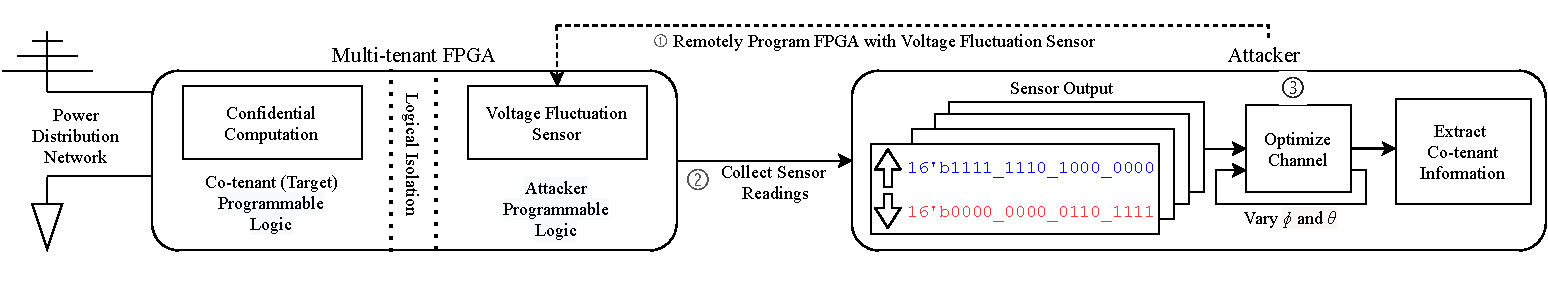
\includegraphics[width=\linewidth]{img/remote-tdc-attack.pdf}
\vspace{-30px}
\caption{Remote TDC Threat Model: \raisebox{.5pt}{\textcircled{\raisebox{-.8pt} {1}}} An attacker is given access to a remote multi-tenant FPGA and programs it with a \sensor. \raisebox{.5pt}{\textcircled{\raisebox{-.8pt} {2}}} The sensor readings are gathered and sent to the attacker for analysis. \raisebox{.5pt}{\textcircled{\raisebox{-.8pt} {3}}} The attacker tunes the parameters $\theta$ and $\phi$ to better extract co-tenant information. This paper studies the impact of $\theta$ and $\phi$ tuning.}

\vspace{-5px}
\label{fig:remote-tdc-attack}
\end{figure*} 


\begin{figure*}[t!]
%\vspace{-20px}
\centering
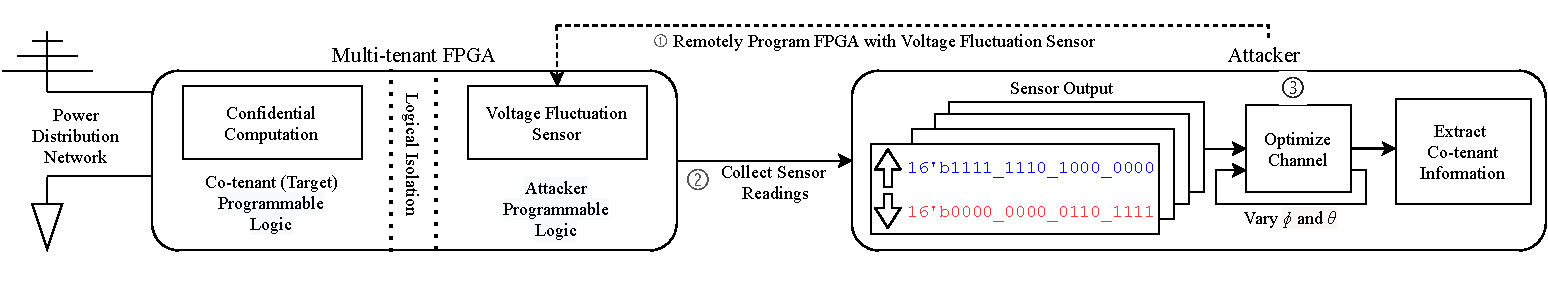
\includegraphics[width=\linewidth]{img/remote-tdc-attack.pdf}
\vspace{-30px}
\caption{Remote TDC Threat Model: \raisebox{.5pt}{\textcircled{\raisebox{-.8pt} {1}}} An attacker is given access to a remote multi-tenant FPGA and programs it with a \sensor. \raisebox{.5pt}{\textcircled{\raisebox{-.8pt} {2}}} The sensor readings are gathered and sent to the attacker for analysis. \raisebox{.5pt}{\textcircled{\raisebox{-.8pt} {3}}} The attacker tunes the parameters $\theta$ and $\phi$ to better extract co-tenant information. This paper studies the impact of $\theta$ and $\phi$ tuning.}

\vspace{-5px}
\label{fig:remote-tdc-attack}
\end{figure*}

The attacker is a malicious adversary that aims to extract information from spatiotemporal co-tenants. This could be as simple as whether a co-tenant is currently using the FPGA, e.g., to know when to launch a fault attack~\cite{gnad2017voltage, krautter2018fpgahammer, sugawara2019oscillator}. The attacker could classify whether a specific type of computation is occurring on the shared FPGA, e.g., is the co-tenant performing encryption? It could infer details about the co-tenant’s design, e.g., are they using a soft processor? Is it a RISC-V processor? The attacker could also learn information about the data being computed upon, e.g., extracting a cryptographic key~\cite{zhao2018fpga, schellenberg2018inside, glamovcanin2020cloud}, and leverage the architectural details learned about implementation to increase recovery speeds.

The attacker can implement a \sensor. Our \sensor is a variant of a TDC sensor~\cite{zick2013sensing}.  %Other \sensors, e.g., those based on ring-oscillators~\cite{boemo1997thermal, zick2012low}, are also potentially feasible with modifications to our framework.  
We assume the sensor will pass bitstream analysis techniques that  detect remote attacks~\cite{krautter2019mitigating}. As discussed later, our sensor passes the checks performed by Amazon AWS F1 instances. %Our sensor does not have timing path violations or combinational cycles; thus, it is significantly less likely to be detected during bitstream analysis than ring oscillator-based sensors.   

We do not make any assumptions about where the sensor is placed, e.g., the victim computation does not need to have one of its wires running through it~\cite{provelengios2019characterizing,giechaskiel2018leaky, ramesh2018fpga}. However, the sensors are more sensitive to computations that are spatially closer~\cite{provelengios2019characterizing, krautter2020cpamap}, and so, as proximity decreases, demand for sensor tuning described in this increases. We consider only attacks within the same programmable logic. However, similar attacks have been shown from the FPGA to a CPU on the same die~\cite{zhao2018fpga}, across dies on a 2.5D integrated package~\cite{giechaskiel2019reading}, and across chips on the same board~\cite{schellenberg2018remote, giechaskiel2020c3apsule}. %Thus, our general techniques could be used for these other scenarios to infer more information about the overall system (granted, they will likely not be as effective due to a reduction in sensor signal to noise).

The shell-role architecture in existing cloud FPGA-as-a-service infrastructures could allow a compromised CSP to act as an attacker. Users who do not trust the CSP could deploy their cloud applications within FPGA trusted execution environments \cite{zhao2022shef}. A compromised CSP may include one or more \sensors within the shell logic to perform side-channel analysis on the enclave cryptographic cores.

%However, the sensors are more sensitive to computations that are spatially closer~\cite{provelengios2019characterizing, krautter2020cpamap}, and thus, the proximity of the target computation can affect our ability to classify information. Increased physical distances reduce the signal-to-noise ratio making the sensor tuning described in this paper even more necessary to extract better information.
%We assume that the attacker has access to a set of representative IP cores they intend to characterize. These IPs do not necessarily need to be the exact IP the attacker will encounter, but they must have similar computational characteristics. The attacker executes the representative IPs alongside a \sensor in a controlled environment to build a corpus of labeled training data for each type of targeted computation. After the training phase, the attacker no longer requires access to the IP cores and is ready to launch the attack remotely.  

%The attacker remotely uploads a bitstream containing a \sensor. The sensor readings are captured and sent back to the attacker for analysis. Our experiments perform classification off the remote FPGA, but we envision a scenario where the attacker performs classification locally, e.g., by implementing a classification engine on the remote FPGA. The gathered sensor readings are transformed into an image and fed into the pre-trained neural network that classifies the computation (as described in Section~\ref{sec:classifier}).
